\documentclass[12pt, letterpaper]{article}

\usepackage[utf8]{inputenc}
\usepackage[spanish, es-tabla]{babel} 
\usepackage{amsmath, amssymb, amsthm} 
\usepackage[svgnames,table]{xcolor}
\usepackage[T1]{fontenc}  
\usepackage{tikz}  
\usepackage{fancyhdr}  
\usepackage{graphicx} 
\usepackage{hyperref} 
\usepackage{enumitem} 

\hypersetup{
    colorlinks=true,
    linkcolor=blue,
    filecolor=magenta,      
    urlcolor=cyan,
}

\usepackage[width=152.6mm, top=1in, bottom=1in, bindingoffset=6mm]{geometry}

\definecolor{burdeos}{HTML}{64293E}
\definecolor{grisc}{HTML}{89888B}
\definecolor{grisCIMAT}{RGB}{137,136,139}  
\definecolor{rojoCIMAT}{RGB}{100,41,62}  

\pagestyle{fancy}
\fancyhf{} 

\renewcommand{\headrulewidth}{0pt} 
\renewcommand{\footrulewidth}{1.5pt} 

\renewcommand{\footrule}{\hbox to\headwidth{\color{rojoCIMAT}\leaders\hrule height \footrulewidth\hfill}}


\fancyfoot[L]{\raisebox{-0.2cm}{
\includegraphics[height=0.65cm]{Cimat_horizontal.png}}}

\fancyfoot[R]{\vspace{0.2cm} \textcolor{grisc}{\textbf{\thepage}}}

\makeatletter 

\setlength{\headheight}{15pt}  

\fancypagestyle{firststyle}{
    \renewcommand{\headrulewidth}{0pt}
    \renewcommand{\footrulewidth}{0pt}
    \fancyhf{}
    \fancyfoot[C]{\begin{tikzpicture}[remember picture,overlay] \node[anchor=south east, yshift=-1.5mm, xshift=1.5mm] at (current page.south east) {
\includegraphics[width=215.9mm]{Cimat_banner.png}}; \end{tikzpicture}}
}

\@ifpackageloaded{geometry}{}{\RequirePackage[pass]{geometry}}

\newcommand*{\documentType}[1]{\gdef\@documentType{#1}}
\newcommand*{\degree}[1]{\gdef\@degree{#1}}
\newcommand*{\cityandyear}[1]{\gdef\@cityandyear{#1}}
\newcommand*{\tutor}[1]{\gdef\@tutor{#1}}

\renewcommand*{\maketitle}{
	\begin{titlepage}
		\newgeometry{left=1.2cm,right=1.2cm,bottom=1.0cm,top=0.9cm}
		\thispagestyle{firststyle} 

        \noindent
        
        \begin{minipage}[c]{0.18\textwidth}
            \begin{flushleft}
                
\includegraphics[height=3.2cm]{Cimat_portada.png}  
            \end{flushleft}
        \end{minipage}
        \begin{minipage}[c]{0.8\textwidth}
            \begin{center}
                {\Large {\color{rojoCIMAT} {\bfseries Centro de Investigación en Matemáticas, A.C.}}}
            \end{center}
        \end{minipage}
        
        \vspace{0.1cm}
        {\color{rojoCIMAT} \hrule height1.3pt} 
        \vspace{3.5cm}  

    	\begin{center}
    	    % Título
    	    {\bfseries \LARGE \scshape\@title\par}
    	    \vspace{2.5cm}
    	    
    	    \makebox[8cm][s]{\Large\bfseries \@documentType }\\[0.2cm]
    	    {\normalsize Trabajo correspondiente al}\\[0.2cm]
    	    {\large \bfseries \@degree}\\[1.5cm]
    
           % Autores
    	    {\bfseries \large Presentan}\\[0.5cm]
    	    {\large \@author}\par
    	    
    	    \vspace{1.5cm} % Espacio entre autores y el tutor
    	    
    	    % Tutor
    	    {\bfseries \large Tutor}\\[0.2cm]
    	    {\large \@tutor}\par
    	    
    	    \vfill
    	\end{center}
	
	    \vspace{1cm}
	
        \begin{flushright}
            {\small \@cityandyear}
        \end{flushright}
    \end{titlepage}
    \restoregeometry 
}
\makeatother 

\begin{document}

% DATOS DE LA PORTADA

\title{FOLIACIÓN PARADÓJICA DE GHYS-TABACHNIKOV-TIMORIN}


\documentType{R E P O R T E}
\degree{Centro de Investigación en Matemáticas}
\cityandyear{Guanajuato, Guanajuato, Julio de 2026}
\tutor{
    \textbf{Néstor Fabián Bravo Hernández}
} 

\author{
    \textbf{Godoy Santiago José Ángel}\\
    \textit{\small Facultad de Ciencias, UNAM}\\[0.5cm]
    \textbf{Martínez Flores Aldo Emiliano}\\
    \textit{\small Unidad Académica de Matemáticas, UAZ}\\[0.5cm]
    \textbf{Ramirez Lefranc Melani Samantha}\\
    \textit{\small Facultad de Ciencias, UNAM}\\ 
}

\maketitle

\newpage

\newpage

\section*{0. ¿Qué necesitas saber?}
Polinomios de Taylor para funciones de una variable, teorema del valor medio, derivadas parciales de aplicaciones de 2 variables, el Teorema de la función inversa para aplicaciones de 2 variables, curvas de nivel de una función de 2 variables, regla de la cadena (para aplicaciones de 2 variables), el gradiente de una función de 2 variables es ortogonal a sus curvas de nivel.

\section*{1. Introducción}
Sea $f : [a,b] \to \mathbb{R}$ una función de clase $C^n$ y $t \in [a,b]$.

\vspace{0.3cm}
\noindent \textbf{\textcolor{burdeos}{Definición 1}} \textit{El polinomio de Taylor de $f$, de grado $n$, centrado en $t$, es:}
\[ p_{n,t}(x) = f(t) + f'(t)(x - t) + \frac{1}{2}f''(t)(x - t)^2 + \cdots + \frac{1}{n!}f^{(n)}(t)(x - t)^n. \]

\noindent \textbf{Nota:} Decir que $f : [a,b] \to \mathbb{R}$ es diferenciable, realmente significa que, de hecho, $f$ está definida (y es diferenciable) en un intervalo abierto $(c,d) \supset [a,b]$.

\vspace{0.4cm}
\noindent \textbf{Ejercicio 1} \textit{Muestra que, para toda $k : 0, 1, \dots, n$, $p_{n,t}^{(k)}(t) = f^{(k)}(t)$.}

Antes de demostrar este ejercicio, demostraremos un lema que se nos será útil posteriormente:\\

\textbf{\textcolor{burdeos}{Lema 1:}} Derivada k-ésima de un monomio desplazado:\\

Sea $g(x) = a(x-t)^i$, donde $a$ y $t$ son constantes.\\

 Si $k=1$, $g'(x) = a \cdot i(x-t)^{i-1}$
 
 Si $k=2$, $g''(x) = a[i(i-1)](x-t)^{i-2}$
 
 Si $k=3$, $g'''(x) = a[i(i-1)(i-2)](x-t)^{i-3}$\\

Asumiendo $k \leq i$:
\[ g^{(k)}(x) = a \cdot [i(i-1)(i-2) \cdots (i-k+1)](x-t)^{i-k} \]
Notemos que:
\[ i(i-1) \cdots (i-k+1) = \frac{i(i-1) \cdots (i-k+1) \cdot (i-k)!}{(i-k)!} = \frac{i!}{(i-k)!} \]
$\implies g^{(k)}(x) = a \frac{i!}{(i-k)!}(x-t)^{i-k}$\\

Si $k=i$, $g^{(i)}(x) = a \frac{i!}{0!}(x-t)^{i-i} = a \cdot i! (x-t)^0 = a \cdot i! = cte$\\

Si continuamos derivando 1 vez más $k > i \implies g^{(k)}(x) = 0$

\begin{proof}[\textbf{\textcolor{teal}{Demostración}}]

    Por def. $p_{n,t}(x) = \sum_{i=0}^{n} \frac{f^{(i)}(t)}{i!}(x-t)^i$
    
    Al derivar $k$ veces con respecto a $x$ en ambos lados: (Por linealidad de la derivada, es igual a la suma de las derivadas de cada término)
    \[ p_{n,t}^{(k)}(x) = \sum_{i=0}^{n} \frac{d^k}{dx^k} \left[ \frac{f^{(i)}(t)}{i!}(x-t)^i \right] \]
    Por el lema 1, donde $a = \frac{f^{(i)}(t)}{i!}$; para $i<k$, la derivada es cero.\\
    Para $i\geq k$
    
    \[ p_{n,t}^{(k)}(x) = \sum_{i=k}^{n} \left[ \frac{f^{(i)}(t)}{i!} \frac{i!}{(i-k)!} (x-t)^{i-k} \right] = \sum_{i=k}^{n} \frac{f^{(i)}(t)}{(i-k)!}(x-t)^{i-k} \]
    Cuando $x=t$:
    \[ p_{n,t}^{(k)}(t) = \sum_{i=k}^{n} \frac{f^{(i)}(t)}{(i-k)!}(t-t)^{i-k} = \sum_{i=k}^{n} \frac{f^{(i)}(t)}{(i-k)!}(0)^{i-k} \]
    Si $i>k \implies i-k>0$, lo que implica que $0^{i-k}=0$, ent. todos los términos posteriores se anulan.\\
    Si $i=k$ ent $i-k=0$. Algebraicamente $0^0 := 1 \implies p_{n,t}^{(k)}(t) = \frac{f^{(k)}(t)}{(k-k)!} = \frac{f^{(k)}(t)}{0!} = f^{(k)}(t)$
    $\therefore p_{n,t}^{(k)}(t) = f^{(k)}(t)$
\end{proof}

\vspace{0.4cm}
\noindent \textbf{Ejercicio 2} \textit{Considera $f(x) = x^3$. Calcula $p_{2,t}(x)$ para toda $t$.}

\begin{proof}[\textbf{\textcolor{teal}{Solución}}]
    Calculamos $p_{2,t}(x)$ de $f(x)=x^3$
    \[ p_{2,t}(x) = f(t) + f'(t)(x-t) + \frac{f''(t)}{2}(x-t)^2 \]
    Calculamos las derivadas necesarias de $f(t)$
    
    $\implies f'(t)=3t^2$
    
    $\implies f''(t)=6t$
    
    $\implies p_{2,t}(x) = t^3 + 3t^2(x-t) + \frac{6t}{2}(x-t)^2 = t^3 + 3t^2x - 3t^3 + 3t(x^2 - 2tx + t^2) = t^3 + 3t^2x - 3t^3 + 3tx^2 - 6t^2x + 3t^3$
    
    $\implies p_{2,t}(x) = 3tx^2 - 3t^2x + t^3$
\end{proof}

\vspace{0.4cm}
\noindent \textbf{Ejercicio 3} \textit{Grafica a mano $f(x) = x^3$ en el intervalo $[-2, 4]$. En el mismo dibujo, también grafica $p_{2,t}$ para $t = \frac{1}{2}, 1, 2$.}


\begin{proof}[\textbf{\textcolor{teal}{Solución}}]
    Para $t=1/2$: $p_{2,1/2}(x) = 3(\frac{1}{2})x^2 - 3(\frac{1}{4})x + \frac{1}{8} = \frac{3}{2}x^2 - \frac{3}{4}x + \frac{1}{8}$
    
    Para $t=1$: $p_{2,1}(x) = 3(1)x^2 - 3(1)x + 1 = 3x^2 - 3x + 1$
    
    Para $t=2$: $p_{2,2}(x) = 6x^2 - 12x + 8$\\
    
    Como demostramos en el problema 1, cada parábola y curva cúbica coinciden en $x=t$
    $f(x)$ en $(1/2, 1/8)$ y $p_{2,1/2}$ en $(1/2, 1/8)$
    $p_{2,1}$ en $(1, 1)$
    $p_{2,2}$ en $(2, 8)$
    
    Dado que estamos aproximando una función cúbica a parábolas, si nos fijamos en su residuo:
    \[ f(x) - p_{2,t}(x) = x^3 - (3tx^2 - 3t^2x + t^3) = (x-t)^3 \]
    Notemos que $(x-t)^3$ cambia de signo al pasar por $t$, entonces la curva atraviesa la parábola exactamente en el punto de tangencia.
\end{proof}

\begin{figure}[h]
    \centering
    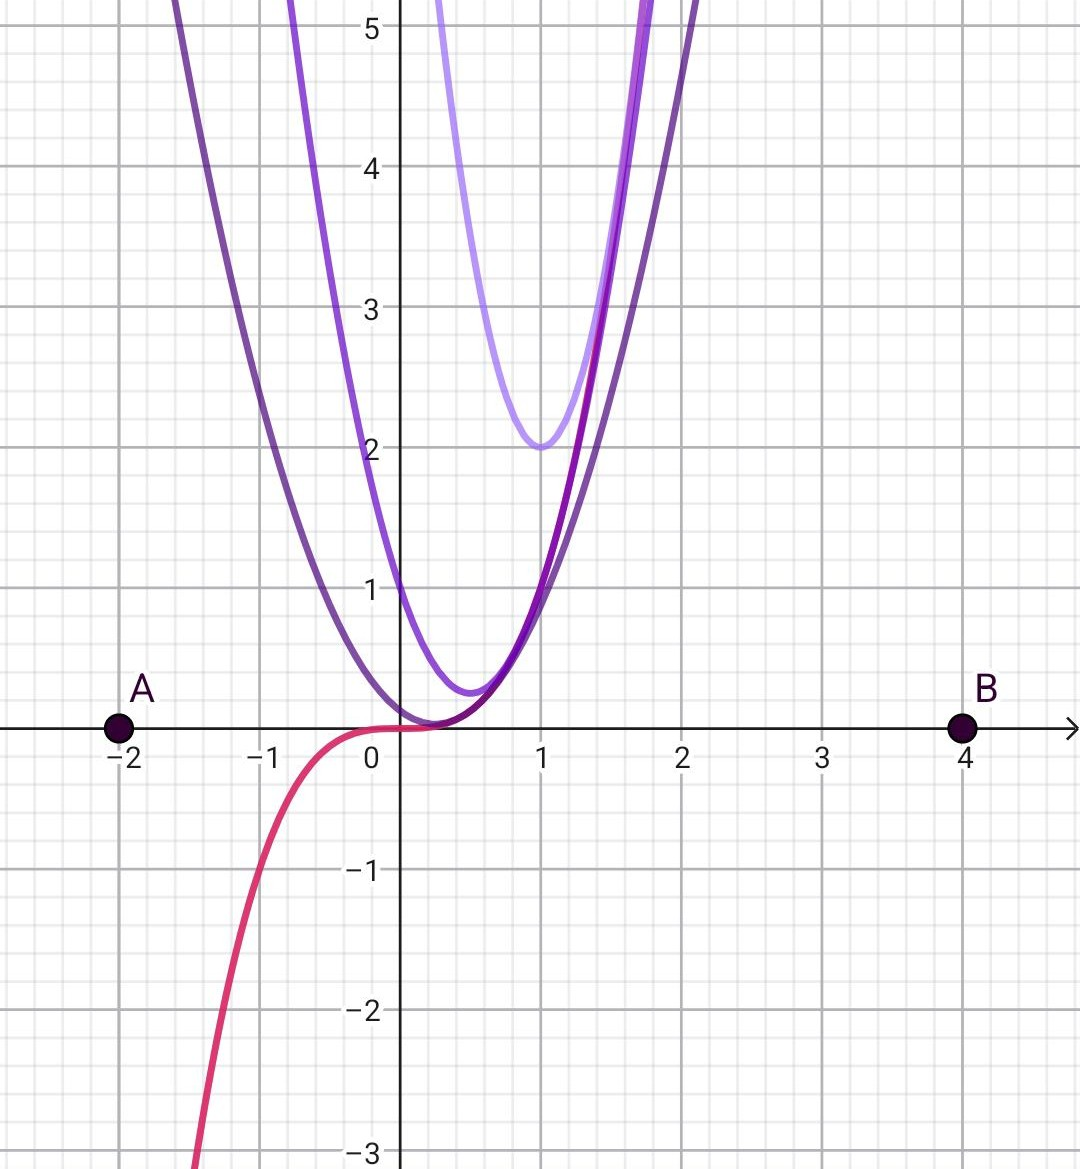
\includegraphics[width=0.5\linewidth]{x_cubica.jpeg}
    \caption{Gráficas de $x^3$ y $p_{2,t}$}
    \label{fig:placeholder}
\end{figure}

\vspace{0.4cm}

\noindent \textbf{Ejercicio 4} \textit{Ahora usa algún programa de computadora para graficar $f(x) = x^3$ (todavía en el intervalo $[-2, 4]$) y $p_{2,t}(x)$ para 50 valores diferentes de $t$. Curiosamente, ¡las gráficas de todos los $p_{2,t}(x)$ no se intersectan! ¿Puedes verlo?}\\

    \begin{figure}[h]
        \centering
        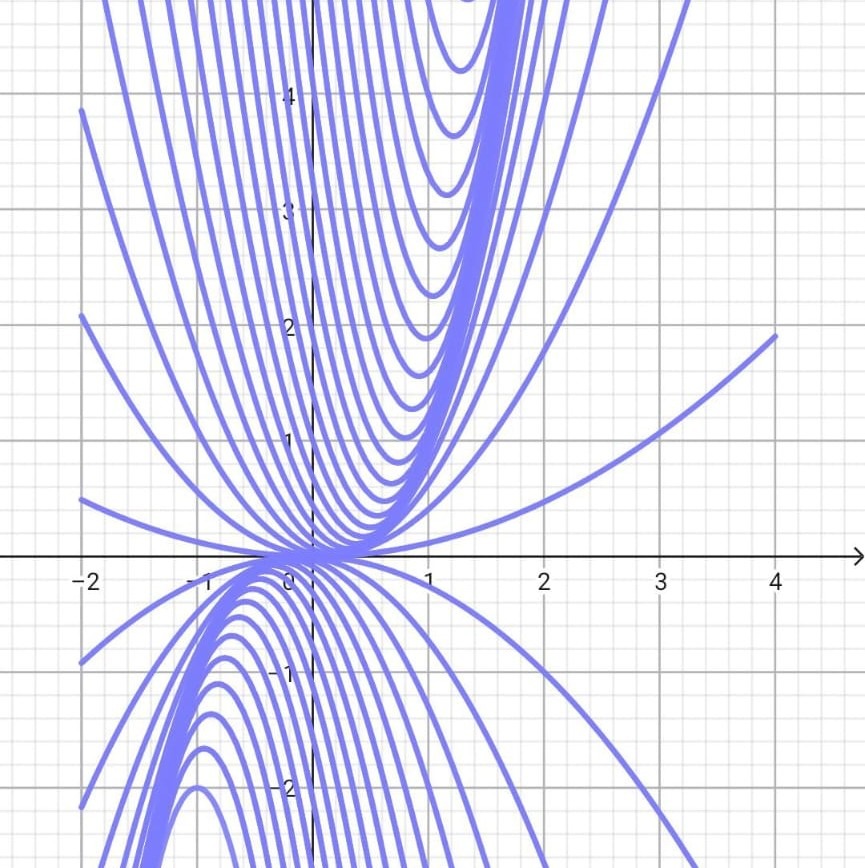
\includegraphics[width=0.5\linewidth]{50_valores.jpeg}
        \caption{Gráficas para 50 valores de t.}
        \label{fig:placeholder}
    \end{figure}
    
    *Los parábolas recorren el plano (lo barren).
    
    *Ninguna parábola interseca a otra parábola (se apilan).


\newpage

\section*{2. El teorema de Ghys-Tabachnikov-Timorin}

\noindent \textbf{\textcolor{burdeos}{Teorema 1 (Ghys-Tabachnikov-Timorin)}} \textit{Sea $f : [a,b] \to \mathbb{R}$ de clase $C^{n+1}$, $n$ un entero positivo \textbf{par} y $p_{n,t}$ el polinomio de Taylor de $f$ de grado $n$, centrado en $t$.}

\textit{Si $f^{(n+1)}(x) > 0$ para toda $x \in [a,b]$, entonces las gráficas de los polinomios $p_{n,t}(x)$ no se intersectarán en toda la recta real: esto es, si $t \neq s$, entonces $p_{n,t}(x) \neq p_{n,s}(x)$ para toda $x \in \mathbb{R}$.}

\vspace{0.4cm}
\noindent \textbf{Ejercicio 5} \textit{Prueba (siguiendo los pasos sugeridos) el teorema.}
\begin{enumerate}[label=(\alph*)]
    \item \textit{Muestra que las gráficas de $p_{n,t}$ y $p_{n,t_0}$ se intersectan si y solo si $p_{n,t}(x) = p_{n,t_0}(x)$, para alguna $x \in \mathbb{R}$.}
    
    \begin{proof}[\textbf{\textcolor{teal}{Demostración.}}]
        Definimos $graph(p_{n,t}) = \{(x,y) \mid x \in \mathbb{R} , y = p_{n,t}(x)\}$
        
        {\textcolor{teal}{P.D}} Las gráficas de dos polinomios con centros distintos $t_1, t_2 \in [a,b]$ se intersecan si $\exists x \in \mathbb{R}$ t.q $p_{n,t_1}(x) = p_{n,t_2}(x)$
        
        {\textcolor{teal}{$\implies$}} Sup. $graph(p_{n,t_1}) \cap graph(p_{n,t_2}) \neq \emptyset$. 
          
        Sea $(x_0, y_0)$ un punto cualquiera t.q $(x_0, y_0) \in graph(p_{n,t_1}) \cap graph(p_{n,t_2})$. 
        
        Por def de intersección, este pto pertenece simultáneamente a ambos conjuntos: Como $(x_0, y_0) \in graph(p_{n,t_1})$, por def $y_0 = p_{n,t_1}(x_0)$. 
        
        Además $(x_0, y_0) \in graph(p_{n,t_2}) \implies y_0 = p_{n,t_2}(x_0)$. 
        
        Dado que $y_0 = y_0$, para que la igualdad de los ptos sea válida $p_{n,t_1}(x_0) = p_{n,t_2}(x_0)$.
        
        {\textcolor{teal}{$\impliedby$}} Sup existe $x_0 \in \mathbb{R}$ donde $p_{n,t_1}(x_0) = p_{n,t_2}(x_0)$.
        
        Sea $y_0 = p_{n,t_1}(x_0) = p_{n,t_2}(x_0)$. 
        
        Como $y_0 = p_{n,t_1}(x_0)$, el par ordenado $(x_0, y_0) \in graph(p_{n,t_1})$. 
        
        Dado que $y_0 = p_{n,t_2}(x_0)$, el mismo par ordenado $(x_0, y_0) \in graph(p_{n,t_2}) \implies (x_0, y_0) \in graph(p_{n,t_1}) \cap graph(p_{n,t_2}) \implies graph(p_{n,t_1}) \cap graph(p_{n,t_2}) \neq \emptyset$.
        
        Concluimos que gráficas de $p_{n,t}$ y $p_{n,t_0}$ se intersectan sii $p_{n,t}(x) = p_{n,t_0}(x)$ para alguna $x \in \mathbb{R}$.
    \end{proof}

    \item \textit{Fija $x \in \mathbb{R}$, $t_0 \in [a,b]$ y define $\phi : [a,b] \to \mathbb{R}$ como}
    \[ \phi(t) = p_{n,t}(x) - p_{n,t_0}(x). \]
    \textit{Verifica que}
    \[ \phi(t) = \sum_{k=0}^{n} \frac{1}{k!} \left[ f^{(k)}(t)(x - t)^k - f^{(k)}(t_0)(x - t_0)^k \right]. \]
    \textit{Explica porqué $\phi$ es una función $C^1$ y prueba que}
    \[ \phi'(t) = \frac{1}{n!}f^{(n+1)}(t)(x - t)^n. \]
    
    \begin{proof}[\textbf{\textcolor{teal}{Demostración.}}]
        Recordando la definición del polinomio de Taylor de grado $n$ en $t$ y $t_0$.
        
        $p_{n,t} = \sum_{k=0}^{n} \frac{1}{k!} f^{(k)}(t)(x-t)^k$ y $p_{n,t_0} = \sum_{k=0}^{n} \frac{1}{k!} f^{(k)}(t_0)(x-t_0)^k$. 
        
        Sustituimos esto en la definición de $\phi(t)$
        
        \begin{center}
            $\phi(t) = p_{n,t}(x) - p_{n,t_0}(x)$
        \end{center}
        
        $\implies \phi(t) = \sum_{k=0}^{n} \frac{1}{k!} f^{(k)}(t)(x-t)^k - \sum_{k=0}^{n} \frac{1}{k!} f^{(k)}(t_0)(x-t_0)^k$
        
        $\implies \phi(t) = \sum_{k=0}^{n} \frac{1}{k!} [f^{(k)}(t)(x-t)^k - f^{(k)}(t_0)(x-t_0)^k]$\\
        
        ¿Por qué $\phi(t)$ es de clase $C^1$ respecto a $t$?
        Observemos los elementos respecto a t:
        
        * $p_{n,t_0}(x)$ es valor cte.
        
        * $(x-t)^k$ es un monomio desplazado de clase $C^\infty$.
        
        * los coeficientes $f^{(k)}(t)$ dependen de las derivadas de orden $k$ desde $k=0$ hasta $n$.
        
        Por hipótesis $f \in C^{n+1}$, entonces $f^{(n)}(t)$ es derivable y su derivada $f^{(n+1)}(t)$ es continua. Entonces $\phi$ es derivable y su derivada es continua. $\implies \phi \in C^1$.
        
        Obtenemos $\phi'(t)$
        Derivamos respecto a $t$:
        \[ \frac{d}{dt} [ \phi(t) ] = \frac{d}{dt} \left[ \frac{f^{(k)}(t)}{k!}(x-t)^k \right] = \frac{f^{(k+1)}(t)}{k!}(x-t)^k - \frac{f^{(k)}(t)}{(k-1)!}(x-t)^{k-1} \]
        Para $k=0$, el término es $f'(t)$. Entonces al expandir la suma de $k=0$ hasta $k=n$:
        \[ \phi'(t) = f'(t) + \sum_{k=1}^{n} \left[ \frac{f^{(k+1)}(t)}{k!}(x-t)^k - \frac{f^{(k)}(t)}{(k-1)!}(x-t)^{k-1} \right] \]
        \[ = f'(t) - f'(t) + \cdots + \frac{f^{(n+1)}(t)}{n!}(x-t)^n \]
        \[ \phi'(t) = \frac{f^{(n+1)}(t)}{n!}(x-t)^n \]
    \end{proof}

    \item \textit{Muestra que $\phi'(t) > 0$ para toda $t \neq x$.}
    
    \begin{proof}[\textbf{\textcolor{teal}{Demostración.}}]
        Análisis de signo. Tenemos tres factores multiplicándose en $\phi'(t)$:
        
        1. $n! > 0$
        
        2. Por hip $f^{(n+1)}(t) > 0 \quad \forall t \in [a,b]$
        
        3. Por hip, $n$ es par. Recordemos que cualquier base elevada a una potencia par resulta en un num. mayor o igual a cero. Es decir, $(x-t)^n \geq 0$
        
        Multiplicando estos elementos, el signo positivo está garantizado $\phi'(t) \geq 0 \quad \forall t \in [a,b]$
        
        Solo si $x=t \implies (x-t)^n=0$. Si $t \neq x$, $\phi'(t)>0$.
    \end{proof}

    \item \textit{Ahora prueba que $\phi$ es una función estrictamente creciente. Concluye el teorema.}
    
    \begin{proof}[\textbf{\textcolor{teal}{Demostración.}}]
        Prueba que $\phi$ es una función estrictamente creciente.
        
        \textbf{\textcolor{burdeos}{Lema 2:}} Para toda $f:[a,b] \to \mathbb{R}$ derivable con $f'(x)>0$ para cada $x \in [a,b]$ ent. $f$ es estrictamente creciente.
        
        \textbf{\textcolor{burdeos}{Dem.}} Sean $x_1, x_2 \in [a,b]$ con $x_1 < x_2$, por TVM en $[x_1, x_2]$ existe $c \in (x_1, x_2)$ t.q. $\frac{f(x_2)-f(x_1)}{x_2-x_1} = f'(c) > 0 \implies f(x_2)-f(x_1)>0 \implies f(x_2)>f(x_1)$
        
        Esto es inmediato, ya que en el inciso anterior demostramos que $\phi'(t)>0$, esto nos garantiza, por Lema 2, que $\phi$ es una función estrictamente creciente.
    \end{proof}
\end{enumerate}

\vspace{0.4cm}
\noindent \textbf{Ejercicio 6} \textit{Prueba que el teorema es cierto suponiendo que $f^{(n+1)}(x) \neq 0$, para toda $x \in [a,b]$.}

\begin{proof}[\textbf{\textcolor{teal}{Demostración.}}]
    Por hip. inicial, sabemos que $f \in C^{n+1}$.
    
    Asumimos que $f^{(n+1)}(x) \neq 0$ en todo el intervalo.
    
    Por Teorema Valor Intermedio, si $f$ continua toma un valor positivo y un valor negativo en un intervalo, forzosamente debe cruzar por el cero.
    
    Si la función nunca toca el cero en un intervalo conexo, es imposible que cambie de signo.
    Entonces la condición $f^{(n+1)}(x) \neq 0$, tenemos los sig. casos:\\
    
    1) $f^{(n+1)}(x) > 0 \quad \forall x \in [a,b]$
    
    2) $f^{(n+1)}(x) < 0 \quad \forall x \in [a,b]$\\
    
    Para 1) se cumple por lo demostrado anteriormente.
    
    Para 2) Suponemos $f^{(n+1)}(x) < 0 \quad \forall x \in [a,b]$:
    
    Definimos $g(x) = -f(x)$. Como $f \in C^{n+1}$ entonces $g \in C^{n+1}$.
    Entonces su derivada (n+1)-ésima es $g^{(n+1)}(x) = -f^{(n+1)}(x)$.
    
    Como $f^{(n+1)}(x) < 0 \implies g^{(n+1)}(x) > 0 \quad \forall x \in [a,b]$.
    
    Definimos los polinomios de Taylor de $g$ como $q_{n,t}$
    
    $\implies q_{n,t}(x) = -p_{n,t}(x)$
    
    Como $g$ cumple con las hip. de nuestro teorema; $n$ par y $g^{(n+1)}(x) > 0$ entonces podemos afirmar que sus gráficas nunca se intersectan.
    
    Para cualesquiera $t_1 \neq t_2$
    $\implies q_{n,t_1}(x) \neq q_{n,t_2}(x) \quad \forall x \in \mathbb{R}$
    $-p_{n,t_1}(x) \neq -p_{n,t_2}(x) \implies p_{n,t_1}(x) \neq p_{n,t_2}(x) \quad \forall x \in \mathbb{R}$.
    
    $\therefore$ Concluimos que el teorema es válido para $f^{(n+1)}(x) \neq 0$.
\end{proof}

\vspace{0.4cm}
\noindent \textbf{Ejercicio 7} \textit{Muestra que el teorema es falso para $n$ \textbf{impar} (¡da un contraejemplo! Haz un dibujo). Sin embargo, prueba que las gráficas de $p_{n,t_1}$ y $p_{n,t_0}$ (digamos para $t_1 > t_0$) no se intersectan en el intervalo $[t_1, \infty)$.}

\begin{proof}[\textbf{\textcolor{teal}{Solución y contraejemplo.}}]
    Sea $f(x) = x^3$ y $n = 1$ (impar)
    
    $\implies f^{(1+1)}(x) = f''(x) = 6x$ tomamos el intervalo $[1,3]$ para cumplir la hipótesis de que $f^{(n+1)}(x) > 0$
    
    Polinomio de grado 1: $p_{1,t}(x) = f(t) + f'(t)(x-t)$
    
    Centrado en 1: $f(1) + f'(1)(x-1) = 1 + 3x - 3 = 3x - 2$
    
    Centrado en 2: $f(2) + f'(2)(x-2) = 8 + 12x - 24 = 12x - 16$\\
    
    Igualamos:
    \begin{align*}
        3x - 2 &= 12x - 16 \\
        3x - 12x &= -16 + 2 \\
        -9x &= -14 \\
        x &= \frac{-14}{-9} \approx 1.55 \quad \text{Pto. de intersección}
    \end{align*}
    
    \textbf{\textcolor{teal}{Dem.}}\\
    $\exists x \in [t_1, \infty)$ t.q $p_{n,t_1}(x) = p_{n,t_0}(x)$
    
    $\implies$ $\Phi(t_1) = p_{n,t_1}(x) - p_{n,t_0}(x) = 0$
    
    $\Phi(t_1) = 0 \qquad \Phi(t_0) = 0$
    
    $\implies \Phi(t_1) = 0 = \Phi(t_0)$
    
    $\exists c \in (t_0, t_1) \quad \Phi'(c) = 0$ \ (Recordando Teorema de Rolle.)
    
    $\Phi'(c) = \frac{1}{n!}f^{(n+1)}(c)(x-c)^n = 0$
    
    $\implies x - c = 0 \iff x = c$ {\textcolor{red}{!  Contradicción.}}
    
    $x$ no puede estar en $[t_1, \infty)$ y $(t_0, t_1)$ al mismo tiempo.
    
    $\therefore$ Las gráficas de $p_{n,t_1}$ y $p_{n,t_0}$ no se intersecan en $[t_1, \infty)$.
\end{proof}

\vspace{0.4cm}
\noindent \textbf{Ejercicio 8} \textit{Bajo las mismas hipótesis del teorema, define una región}
\[ U = \{ (x,y) \in \mathbb{R}^2 \mid x \in \mathbb{R}, \text{ y entre } p_{n,a}(x) \text{ y } p_{n,b}(x) \} \]

\begin{figure}[h]
    \centering
    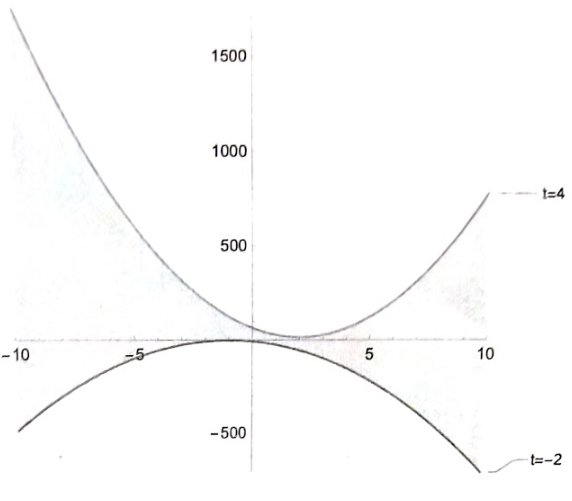
\includegraphics[width=0.7\linewidth]{Ej_8.png}
    \caption{La región $U$, para $f(x) = x^3$ en el intervalo $[-2, 4]$}
    \label{fig:placeholder}
\end{figure}

\noindent Define $\Phi : \mathbb{R} \times [a,b] \to U$ como
\[ \Phi(x,t) = (x, p_{n,t}(x)). \]

\begin{enumerate}[label=(\alph*)]
    \item \textit{Verifica que $\Phi$ manda cada línea horizontal $t = \text{constante}$ sobre la gráfica de $p_{n,t}$.}
    
    \begin{proof}[\textbf{\textcolor{teal}{Demostración.}}]
        Sea $L_{t_0} = \{ (x, t_0) \mid x \in \mathbb{R} \}$ la línea horizontal de $t_0 \in [a,b]$ y $Graph(p_{n,t_0})$ dicha gráfica. Entonces
        \[ \Phi[L_{t_0}] = \{ \Phi(x, t_0) \mid x \in \mathbb{R} \} \]
        \[ = \{ (x, p_{n,t_0}(x)) \mid x \in \mathbb{R} \} = Graph(p_{n,t_0}) \]
    \end{proof}
    
    \item \textit{Prueba que en verdad $\Phi(x,t) \in U$, para toda $(x,t) \in \mathbb{R} \times [a,b]$.}
    
   \begin{proof}[\textbf{\textcolor{teal}{Demostración.}}]
        i.e $Im \Phi \subseteq U$.
        Recordemos la función $\phi : [a,b] \to \mathbb{R}$, con $t_0$ fijo, definida como $\phi(t) = p_{n,t}(x) - p_{n,t_0}(x)$ y notemos que $\phi'(t) = \frac{d}{dt}(p_{n,t}(x))$, pues $p_{n,t_0}(x)$ es constante y, gracias a 5.c) sabemos que $\phi'(t) > 0$, entonces $p_{n,t}(x)$ como función de $t$ es creciente. Por lo tanto, si $a \leq t \leq b$ tenemos
        \[ p_{n,a}(x) \leq p_{n,t}(x) \leq p_{n,b}(x) \text{ para toda } x \in \mathbb{R}. \]
        Ahora si $(x,t) \in \mathbb{R} \times [a,b]$ se cumple $\Phi(x,t) = (x, p_{n,t}(x))$ con $x \in \mathbb{R} \land p_{n,a}(x) \leq p_{n,t}(x) \leq p_{n,b}(x)$ se sigue que $\Phi(x,t) \in U$
    \end{proof}
    
    \item \textit{Prueba (es inmediato) que $\Phi$ es 1-1.}
    
    \begin{proof}[\textbf{\textcolor{teal}{Demostración.}}]
        Supongamos $(x,t)$ y $(x_0, t_0)$ en $\mathbb{R} \times [a,b]$ tales que
        \[ \Phi(x,t) = \Phi(x_0, t_0) \implies (x, p_{n,t}(x)) = (x_0, p_{n,t_0}(x_0)) \]
        \[ \implies x = x_0 \land p_{n,t}(x) = p_{n,t_0}(x_0) \]
        Esto es $p_{n,t}(x) = p_{n,t_0}(x)$, el Teorema 1 asegura que $t = t_0$. Finalmente $(x,t) = (x_0, t_0)$
    \end{proof}
    
    \item \textit{Ahora demuestra que $\Phi$ es sobre $U$.}
    
   \begin{proof}[\textbf{\textcolor{teal}{Demostración.}}]
        Sea $(x,y) \in U$ por la definición de $U, x \in \mathbb{R}$ y $p_{n,a}(x) \leq y \leq p_{n,b}(x)$, también $0 \leq y - p_{n,a}(x) \leq p_{n,b}(x) - p_{n,a}(x)$.
        
        Tomemos la función continua $\Phi_{xa} : [a,b] \to \mathbb{R}$ dada por
        \[ \Phi_{xa}(t) = p_{n,t}(x) - p_{n,a}(x) \]
        Y veamos que $\Phi_{xa}(a) = 0 \leq y - p_{n,a}(x) \leq \Phi_{xa}(b)$.
        
        Entonces el Teorema del valor intermedio asegura la existencia de $t_0 \in [a,b]$ tq $\Phi_{xa}(t_0) = y - p_{n,a}(x)$ i.e $p_{n,t_0}(x) - p_{n,a}(x) = y - p_{n,a}(x) \implies y = p_{n,t_0}(x)$.
        Ahora
        \[ \Phi(x, t_0) = (x, p_{n,t_0}(x)) = (x, y) \]
    \end{proof}
    
    \item \textit{¿Será cierto que $\Phi$ es $C^1$? En otras palabras, ¿es $C^1$ como función de $x$ y como función de $t$?}
    
   \begin{proof}[\textbf{\textcolor{teal}{Demostración.}}]
        Usando $\Phi(x,t) = (x, p_{n,t}(x))$
        Encontramos las derivadas parciales de las coordenadas de $\Phi$\\
        
        $\frac{\partial}{\partial x} \Phi_1 = \frac{d}{dx} x = 1$
        
        $\frac{\partial}{\partial t} \Phi_1 = \frac{d}{dt} x = 0$
        
        $\frac{\partial}{\partial x} \Phi_2 = \frac{\partial}{\partial x} p_{n,t}(x) = p'_{n,t}(x)$\\
        
        Consideremos $\Phi_{xa} : [a,b] \to \mathbb{R}$, $\Phi_{xa}(t) = p_{n,t}(x) - p_{n,a}(x)$ para un $x$ fijo, con los resultados del ejercicio 5
        $\frac{\partial}{\partial t} p_{n,t}(x) = \frac{d}{dt} \Phi_{xa}(t) = \Phi'_{xa}(t) = \frac{1}{n!} f^{(n+1)}(t)(x-t)^n$
        
        Ya que $\Phi_{xa}$ es $C^1$, $\frac{\partial}{\partial t} \Phi_2 = \frac{\partial}{\partial t} p_{n,t}(x)$ es continua.
        Por lo que las 4 derivadas parciales son continuas y $\Phi$ es $C^1$.
    \end{proof}
\end{enumerate}

\noindent \textit{Decimos que $U$ está foliado por las gráficas de los polinomios $p_{n,t}$, $t \in [a,b]$.}


\begin{figure}[h]
    \centering
    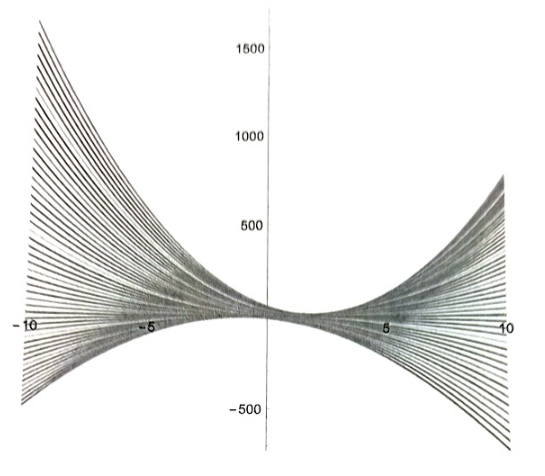
\includegraphics[width=0.7\linewidth]{Ej_9.png}
    \caption{$U$ foliado por las gráficas de los $p_{n,t}$, $t \in [a,b]$}
    \label{fig:placeholder}
\end{figure}


\vspace{0.4cm}
\noindent \textbf{Ejercicio 9} \textit{Como $\Phi : \mathbb{R} \times [a,b] \to U$ es biyectiva, su inversa $\Phi^{-1} : U \to \mathbb{R} \times [a,b]$ existe ($\Phi^{-1}$ es la aplicación que endereza las gráficas de los polinomios de Taylor $p_{n,t}$, de $f$). Prueba que $\Phi^{-1}$ es de la forma}
\[ \Phi^{-1}(x,y) = (x, F(x,y)) \]
\textit{para alguna función $F : U \to [a,b]$.}

\begin{proof}[\textbf{\textcolor{teal}{Demostración.}}]
    Sean $\pi_1, \pi_2 : \mathbb{R}^2 \to \mathbb{R}$ las proyecciones de las coordenadas.
    
    Definimos una función $F = \pi_2 \circ \Phi^{-1} : U \to \mathbb{R}$
    
    * Notemos que $Im F \subseteq [a,b]$ pues $\pi_2[\mathbb{R} \times [a,b]] = [a,b]$
    
    Llamemos $(x_1, t) = \Phi^{-1}(x,y)$ para algún $(x,y) \in U$. Aplicando $\pi_2$ en ambos lados
    $t = \pi_2(x_1, t) = \pi_2(\Phi^{-1}(x,y)) = F(x,y)$
    
    Además $(x,y) = \Phi(x_1, t) = (x_1, p_{n,t}(x_1)) \implies x = x_1$.
    
    Por lo tanto $\Phi^{-1}(x,y) = (x_1, t) = (x, F(x,y))$
\end{proof}

\vspace{0.4cm}
\noindent \textbf{Ejercicio 10} \textit{Demuestra que $F(x,y) = t$ si y solo si $p_{n,t}(x) = y$. En otras palabras, $F(x,y)$ es el número $t$ donde el polinomio de Taylor de $f$ (cuya gráfica pasa por $(x,y)$) está centrado.}

\begin{proof}[\textbf{\textcolor{teal}{Demostración.}}]
    Como $\Phi^{-1}(x,y) = (x, F(x,y))$
    
    $F(x,y) = t \iff \Phi^{-1}(x,y) = (x,t) \implies (x,y) = \Phi(x,t) \implies (x,y) = (x, p_{n,t}(x)) \implies y = p_{n,t}(x)$
    
    Ahora bien, definimos $F^{-1}[\{t\}]$ como la preimagen de $F$, esto es el conjunto de todos los puntos $(x,y)$ t.q. $F(x,y)=t$. 
    
    Acabamos de demostrar que $F(x,y) = t \iff y = p_{n,t}(x)$, entonces el conjunto $F^{-1}[\{t\}]$ son los puntos $y = p_{n,t}(x)$.
    
    La región $U$ está foliada, porque a cada punto le toca un solo valor $t$, así que por cada punto pasa una sola curva de nivel, es decir, una sola gráfica del polinomio. (La curva de nivel $F^{-1}(t) = graph(p_{n,t}(x))$).
\end{proof}

\vspace{0.4cm}
\noindent \textbf{Ejercicio 11} \textit{Describe la imagen de la gráfica de $f$ bajo $\Phi^{-1}$ (sabemos que las rectas horizontales, en $\mathbb{R} \times [a,b]$, son mandadas por $\Phi$ sobre las gráficas de los polinomios de Taylor $p_{n,t}$; ¿así que, qué curva en $\mathbb{R} \times [a,b]$ se aplica (bajo $\Phi$) sobre la gráfica de $f$?).}

\begin{proof}[\textbf{\textcolor{teal}{Demostración.}}]
    {\textcolor{teal}{P.D.}} Qué curva en el dominio $(x,t)$ se convierte en la gráfica de $f$ al aplicarle $\Phi$.
    
    Definimos $Graph(f) = \{(x, f(x))\}$. 
    
    Sea $(x,t) \in \mathbb{R} \times [a,b]$ tales que $\Phi(x,t) = (x, f(x))$. 
    
    Por definición $\Phi(x,t) = (x, p_{n,t}(x)) \implies f(x) = p_{n,t}(x)$.
    
    Por el teorema de Taylor, utilizamos la forma de Lagrange para el residuo: $f(x) = p_{n,t}(x) + R_{n}(x) \implies f(x) - p_{n,t}(x) = \frac{f^{(n+1)}(\xi)}{(n+1)!}(x-t)^{n+1}$ para algún $\xi$ entre $x$ y $t$.
    
    Para que la igualdad se cumpla, el residuo tiene que ser 0.
    
    $\implies \frac{f^{(n+1)}(\xi)}{(n+1)!}(x-t)^{n+1} = 0$. 
    
    Por hipótesis inicial $f^{(n+1)} > 0$, entonces la única manera de que sea cero es que $x-t=0 \implies x=t$.
    
    Los únicos puntos en el dominio $\mathbb{R} \times [a,b]$ que mapean a la gráfica de $f$ son aquellos donde $x=t$.
    $\Phi^{-1}[graph(f)] = \{(x,t) \in \mathbb{R} \times [a,b] \mid f(x) = p_{n,t}(x)\}$.
\end{proof}

\vspace{0.4cm}
\noindent \textbf{Ejercicio 12} \textit{Prueba que la gráfica de $f$ intersecta la gráfica de cada $p_{n,t}$ exactamente una vez. Más aún, muestra que en el punto de intersección ambas gráficas son tangentes.}

\begin{proof}[\textbf{\textcolor{teal}{Demostración.}}]
    {\textcolor{teal}{P1}} Intersección. 
    
    Fijamos $t$, buscaremos comparar la gráfica de cada $p_{n,t}(x)$ con $f(x)$. 
    
    Para hallar las intersecciones $\implies f(x) = p_{n,t}(x)$. 
    
    Como demostramos en el ej 11, esta igualdad se da solo cuando $x=t$. 
    
    Las gráficas se cruzan en un solo punto: $(t, f(t))$.
    
    {\textcolor{teal}{P2}} Tangencia. Recordando el ejercicio 1, demostramos que la derivada k-ésima de la función en $x=t$ coincide con la derivada k-ésima del polinomio de Taylor.
    
    $\implies p_{n,t}^{(1)}(t) = f^{(1)}(t) \implies p'_{n,t}(t) = f'(t)$.
    
    Como ambas gráficas pasan por el mismo punto $(t, f(t))$ y tienen exactamente la misma derivada $f'(t)$ en el punto, las gráficas son tangentes.
\end{proof}

\vspace{0.4cm}
\noindent \textbf{Ejercicio 13} \textit{Considera el siguiente argumento ``contradictorio'':}

\noindent \textit{Define $g(x) = F(x, f(x))$, $x \in [a,b]$. Deriva $g$ usando la regla de la cadena:}
\[ g'(x) = \nabla F(x, f(x)) \cdot (1, f'(x)). \]

\noindent \textit{Aseguramos que $g'(x) = 0$:}
\begin{itemize}
    \item \textit{En primer lugar, $\nabla F$ es perpendicular a todas las curvas de nivel (¿por qué?);}
    \item \textit{luego, $\nabla F(x, f(x))$ es perpendicular a la curva de nivel que pasa por $(x, f(x))$;}
    \item \textit{pero en el punto $(x, f(x))$, la curva de nivel (ie. la gráfica de algún $p_{n,t}$) y la gráfica de $f$ son tangentes;}
    \item \textit{luego, $\nabla F(x, f(x)) \cdot (1, f'(x)) = 0$}
\end{itemize}

\noindent \textit{Como $g'(x) = 0$, para toda $x$, $g$ es constante. Pero esto implica que $(x, f(x))$ (ie. la gráfica de $f$) queda contenida en una de las curvas de nivel de $F$. Pero esto es \textbf{absurdo}, ya que sabemos que la gráfica de $f$ intersecta a \textbf{todas} las curvas de nivel.}

\vspace{0.3cm}
\noindent \textit{¿Dónde está el error en el argumento? ¿Cómo resolvemos esta paradoja?}

\begin{proof}[\textbf{\textcolor{teal}{Solución.}}]
    ¿Por qué el argumento falla?
    El argumento asume que $\nabla F$ existe en $(x, f(x))$ para $x \in [a,b]$ probaremos que esto es falso.
    Usando las derivadas parciales de $\Phi$ en un punto $(x,t)$ y veamos que su matriz jacobiana
    \[ J_\Phi(x,t) = \begin{pmatrix} 1 & 0 \\ p'_{n,t}(x) & \frac{1}{n!}f^{(n+1)}(t)(x-t)^n \end{pmatrix} \]
    Y que $\det(J_\Phi(x,x)) = \det \begin{pmatrix} 1 & 0 \\ p'_{n,x}(x) & 0 \end{pmatrix} = 0$ para cada $x \in [a,b]$
    Esto quiere decir que el operador "$D\Phi(x,x)$" no es invertible.
    Como $\Phi^{-1}(x,y) = (x, F(x,y))$, su matriz jacobiana es
    \[ J_{\Phi^{-1}}(x_0,y_0) = \begin{pmatrix} 1 & 0 \\ F_x(x_0,y_0) & F_y(x_0,y_0) \end{pmatrix} = \begin{pmatrix} 1 & 0 \\ & \nabla F(x_0,y_0) & \end{pmatrix} \]
    Donde $F_x$ y $F_y$ son las derivadas parciales de $F$. La existencia de $J_{\Phi^{-1}}(x_0,y_0)$ está ligada a la de $\nabla F(x_0,y_0)$. Esto es, existe $\nabla F$ en $(x_0,y_0)$ si y solo si existe el operador $D\Phi^{-1}(x_0,y_0)$ que es equivalente a decir que $\Phi^{-1}$ es derivable en $(x_0,y_0)$.
    
    Como última propiedad veamos que
    \[ \Phi(x,x) = (x, p_{n,x}(x)) = (x, f(x)) \]
    
    Ahora supongamos que $\Phi^{-1}$ es derivable en $(x, f(x))$, por lo que $D\Phi^{-1}(x, f(x)) = D\Phi^{-1}(\Phi(x,x))$ existe.
    Como $(\Phi^{-1} \circ \Phi)(x,x) = (x,x) \quad \forall x \in [a,b]$
    Podemos derivar con regla de la cadena y obtener
    \[ D\Phi^{-1}(\Phi(x,x)) \circ D\Phi(x,x) = \text{Id} \]
    \[ D\Phi^{-1}(x, f(x)) \circ D\Phi(x,x) = \text{Id} \]
    Entonces $D\Phi(x,x)$ es invertible, una contradicción por lo dicho anteriormente. Finalmente podemos concluir que $\Phi^{-1}$ no es derivable en $(x, f(x))$, luego, $\nabla F(x, f(x))$ no existe.
\end{proof}

\end{document}